\documentclass[12pt,a4paper]{article}
\usepackage{times}
\usepackage[utf8]{inputenc}
%\usepackage[english]{babel}
\usepackage[portuguese]{babel}
\usepackage[T1]{fontenc}
\usepackage{cite}
\usepackage{amsmath,amsfonts,amssymb} % pacote matematico
\usepackage{array}
\usepackage{graphicx,wrapfig}
\usepackage{float}
\usepackage{indentfirst}
\usepackage[inline]{enumitem}

\usepackage{psfrag}
\usepackage{pstricks}
\usepackage{epsfig}
\usepackage{url}           % Legenda no texto e na Lista de figuras diferentes. Habilita \cite{} na legenda.

\setlength{\parindent}{1.2cm}
\setlength{\parskip}{.2cm}
\setlength{\oddsidemargin}{0.5cm}    % Há um offset obrigatorio de
\setlength{\evensidemargin}{0.0cm}   % 1 inch do lado esquerdo e no
\setlength{\topmargin}{-1.2cm}       % topo da folha
\setlength{\headsep}{1.0cm}
\setlength{\textwidth}{15.5cm}
\setlength{\textheight}{24.2cm}
\renewcommand{\baselinestretch}{1.2}
\renewcommand{\labelitemi}{\tiny{\textbullet}}  % Define o ícone principal do itemize

%\hyphenation{Trans-ac-tions}


\begin{document}
\pagenumbering{roman}

\begin{titlepage}
\thispagestyle{empty}
\begin{center}
\large{\bf{UFBA - Universidade Federal da Bahia}} \\
\large{\bf{Graduação em Engenharia da Computação}} \\
\end{center}
\vfill

\centering
\textbf{{\LARGE PLANO DE TRABALHO}}  \\ \vspace{0.5cm}
{\LARGE Graduação}
\vfill




\textbf{{\Large Robô de inspeção com visão imersiva}} \\ %\vspace{0.3cm}
%\hrulefill \\
\vfill
\begin{flushleft}
\textbf{Aluno}: Raffaello Salvetti Santos \hfill{}\\
\textbf{Orientador}: --- \hfill{}\\
\textbf{Linha de Pesquisa}: Robótica {\it ou} Sistemas Robóticos \hfill{}\\
\end{flushleft}

\vfill


\vspace{\stretch{1}}
\begin{center}
\large{\bf{\today}}
\end{center}
\end{titlepage}


\pagenumbering{arabic}

\begin{abstract}
	Inspeção de áreas de difícil acesso ou que apresentam perigo, como dutos de ventilação, subestações de energia elétrica e reservatórios de produtos corrosivos, é uma realidade na indústria. O uso de robôs operados remotamente é uma solução que oferece segurança ao operador. O objetivo deste trabalho é desenvolver um robô remotamente controlado visando eficiência, versatilidade e baixo custo de produção.
\end{abstract}


%---------------------------------------------------------------------------------------------------------
\section{Introdução}
	Dutos de ventilação usados nos sistemas de ar-condicionado estão sujeitos a diversos tipos de danos, dentre os quais pode-se listar os entupimentos progressivos devido ao acúmulo de poeira e acúmulo de pequenos animais mortos. Por normalmente ser locais de pouco acesso, apresentam dificuldades em sua manutenção, favorecendo a proliferação de bactérias e transmissão de vírus\cite{carmo1999qualidade}\cite{bortoletto2002contaminaccao}.\par
	Subestações de energia elétrica, em grande parte das vezes, ficam expostas a intempéries, que causam oxidações em suportes, equipamentos e cabos. Sua inspeção oferece riscos a vida por expor o corpo humano a uma quantidade enorme de energia, apesar de existir norma rigorosa para a realização de inspeções preventivas, acidentes com vítmas ainda acontecem\cite{santos2012inspeccao}.\par
	A inspeção de reservatórios de produtos químicos requer uma minuciosa análise estrutural, uma busca por áreas oxidadas e falhas em pontos de solda, que demanda muito tempo. A exposição a gases e vapores tóxicos, por menor que seja a quantidade, causam riscos a saúde do inspetor\cite{souza2012inspeccao}\cite{molina2008metodo}.\par
	Os exemplos acima, são apenas algumas das atividades extremamente necessárias no ambiente industrial, que expõem pessoas a riscos de morte e que podem ser evitados através de dispositivos especializados. Os dispositivos usados para esse fim, são robôs equipados com ferramentas adequadas para cada tarefa que podem oferecer um sistema de navegação autônomo ou de controle remoto.

%----------------------------------------------------------------------------------------------------------------------
\section{Objetivo}
	O objetivo deste trabalho é a construção de um robô que será controlado remotamente através de um joystick. O dispositivo oferecerá uma visão imersiva, através de uma câmera embarcada, que funcionará em ambientes iluminados ou com pouca luz e tem eixos livres nas direções horizontal e vertical; possuirá também uma câmera localizada na parte traseira do robô que permitirá realizar manobras com mais precisão; Será possível coletar informações do ambiente ao redor do robô através de sensores embarcados como: dois sensores de temperatura, um localizado na "cabeça" do robô (sensor laser), que pode ser direcionado, e outro no corpo do dispositivo; sensor de umidade do ar, sensor de partículas em suspensão no ar e etc. As leituras dos sensores serão apresentadas na tela de navegação do robô e poderão ser enviadas pela rede para um outro operador em tempo de coleta. Através dos dados enviados pela rede, poderá ser montado um mapa, com o auxilio de um software especializado, do local onde o robô se encontra.

%---------------------------------------------------------------------------------------------------------
\section{Metodologia}
	Para o desenvolvimento do robô, será usado uma plataforma feita em alumínio, o chassi, que deverá suportar o peso da bateria, motores, correntes, câmeras e eletrônica necessária para seu funcionamento.\par
	O movimento do robô se dará através de dois motores em conjunto com um par de correntes, acionados por uma placa microcontrolada, especialmente desenhada para esse propósito, que aciona os motores através de PWM\footnote{Modulação por largura de pulso.}. A mesma placa que controla os motores de locomoção, controlará os motores que movimentarão a câmera frontal. A comunicação entre a placa de controle de motores e o sistema computacional embarcado, um \emph{Raspberry PI 1 modelo B}\footnote{Um micro computador do tipo SOC, do inglês "System on a Chip", ou computador num único chip.}, acontecerá através do protocolo $I^2C$.\par
	O software de operação consistirá de módulos que serão desenvolvidos usando o ROS\footnote{Do inglês, Robot Operating System ou Sistema Operacional de Robôs.}. O desenvolvimento dos módulos ROS será feito de forma independente da parte física do robô pois será usado um simulador de ambiente para esse fim.\par
	Os módulos serão: \begin{enumerate*} \item um aplicativo que deverá rodar num celular Android, responsável por mostrar as imagens e sons capturados pelas câmeras embarcadas e fará a ponte de comunicação entre os comandos originados de um joystick bluetooth e a plataforma robótica; \item \label{mod:board} um programa que rodará embarcado numa placa microcontrolada customizada e fará o controle dos motores de locomoção, motores da câmera frontal e a coleta de dados dos sensores; \item um programa rodará num Raspberry PI, responsável por capturar as images das câmeras frontal e traseira, e usará o módulo \ref{mod:board} como interface entre os periféricos; e por fim, \item um programa que rodará num computador remoto, responsável por armazenar dados, gerenciar a conexão entre os módulos e plotar um mapa virtual do caminho percorrido pelo robô.\end{enumerate*}\par

\subsection{Diagrama de blocos}
\begin{figure}[H]
	\centering
	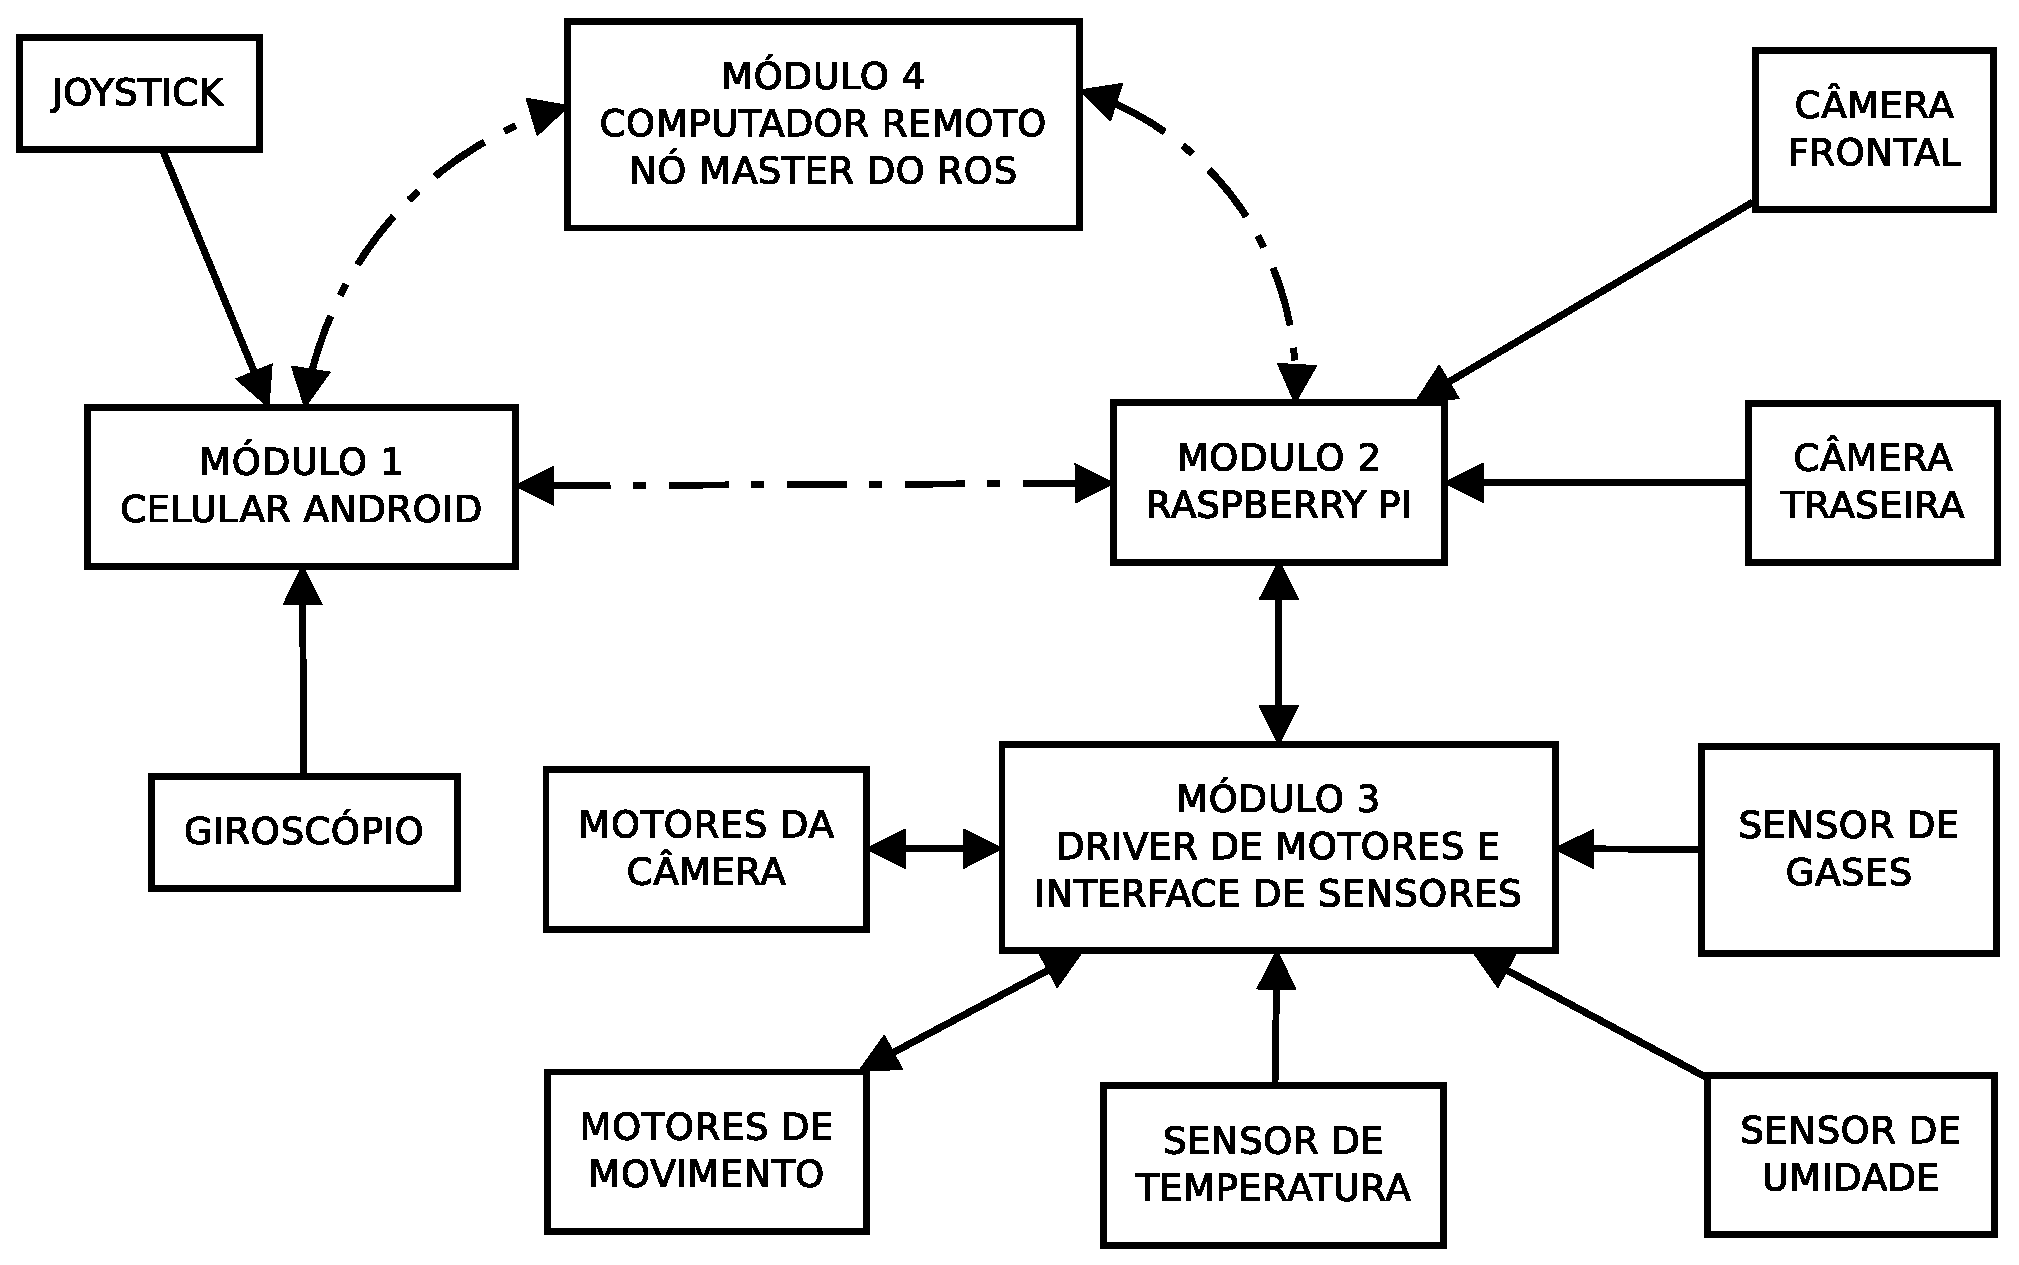
\includegraphics[scale=0.45]{diagrama-modulos} 
	\label{fig:diag-modulos}
	\caption{Diagrama de blocos dos módulos que compõem o robô.}
\end{figure}

\subsection{Descrição dos módulos \label{sec:desc-modulos}}
\begin{enumerate}
\item \textbf{Módulo do Celular Android - Visualização Imersiva\label{mod:celular}}\\
	Esse módulo será um nó do ROS que mostrará as imagens coletadas pelas câmeras embarcadas no robô, módulo \ref{mod:raspi}, e processadas pelo nó master, módulo \ref{mod:ros-master}. Será usado um celular juntamente com um \emph{óculos VR}\footnote{Óculos de realidade virtual.} como um display para mostrar o vídeo e o som transmitido pelas câmeras, dando a ideia de imersão. O módulo deve enviar os dados do giroscópio do celular afim de movimentar a câmera frontal de acordo com o movimento da cabeça do operador. Um joystick comum, que oferece conectividade bluetooth, será usado para movimentar as esteiras do robô e navegar entre as \emph{opções de menu}\footnote{Controle de sensores e luzes.} que aparecem no visor do celular.
\item \textbf{Módulo de Controle Embarcado - Raspberry PI\label{mod:raspi}}\\
	Esse módulo será um nó ROS que rodará num Raspberry PI 1 modelo B, que possui um processador \emph{ARM}\footnote{Do inglês, Advanced RISC Machine. É uma arquitetura de processadores com um numero reduzido de instruções e de baixo custo de produção.} de 700MHz, 512Mb de memória RAM, 26 \emph{GPIO}\footnote{Pinos de propósito geral.}, duas portas USB e uma porta Ethernet. Será responsável por enviar as imagens das câmeras frontal e traseira, lidar com as conexões de rede ethernet (através de cabo umbilical) ou wi-fi, enviar os dados de navegação gerados pelo módulo \ref{mod:celular} para o módulo \ref{mod:motor-driver} e enviar dados dos sensores capturados pelo módulo \ref{mod:motor-driver} para os módulos \ref{mod:celular} e \ref{mod:ros-master}. A comunicação entre o módulo \ref{mod:motor-driver} e o Raspberry PI acontecerá pelos pinos GPIO reservados para a comunicação $I^2C$.
\item \textbf{Módulo Driver - Controlador de Motores e Interface de Sensores\label{mod:motor-driver}}\\
	O módulo drive será uma placa de circuito impresso que possui um microcontrolador \emph{AVR}\footnote{AVR é uma família de microcontroladores que oferece diversos modelos com diversas configurações} ou \emph{PIC}\footnote{PIC é uma família de microcontroladores que oferece diversos modelos com diversas configurações} com periféricos, memória e quantidade de pinos suficientes para realizar suas tarefas. A placa driver terá as seguintes funções: \begin{enumerate*} \item monitorar a tensão da bateria; \item fazer a regulação da tensão de 12V para 5V, tensão que alimenta o Raspberry PI; \item acionar os dois motores das esteiras e os dois  motores da câmera frontal; \item coletar dados dos diversos sensores embarcados; \item controlar as luzes usadas na iluminação do ambiente\end{enumerate*}. A placa possuirá um display indicativo para depuração e status do robô, e um conector do tipo header de duas linhas com 26 pinos, usado para a conexão com os GPIOs do Raspberry PI.
\item \textbf{Módulo Principal - ROS Master\label{mod:ros-master}}\\
	O módulo \ref{mod:ros-master} deverá rodar em um computador com adequado poder de processamento. Para o caso em questão, será um notebook com requisitos de hardware suficientes para rodar o ROS e ser o nó master, rodar processamentos do \emph{Open CV}\footnote{Do inglês, Open Source Computer Vision Library. Uma coleção de aplicativos e bibliotecas para trabalhar com visão computacional e aprendizado de máquinas.} para o reconhecimento de imagens e recurso suficiente para plotar um mapa virtual do trajeto executado pelo robô. 
\end{enumerate}

\subsection{Conhecimento Necessário}
	Para construir os módulos listados na seção \ref{sec:desc-modulos}, se faz necessário os seguintes conhecimentos:
\begin{enumerate}[noitemsep]
	\item Eletrônica Geral
	\item Microcontroladores
	\item Protocolos de Comunicação (\emph{SPI}\footnote{Do inglês, Serial Peripheral Interface ou Interface Periférica Serial. É um protocolo de comunicação serial.} e $I^2C$)
	\item Fontes de Alimentação
	\item Supressão de Ruído (Interferência Eletromagnética)
	\item Acionamento de Motores
	\item Sistemas de Transmissão Mecânica (Corrente de Transmissão)
	\item Sistema Operacional Linux
	\item Sistema Operacional de Robôs - ROS
	\item Sistema Operacional Android
	\item Linguagens de Programação (C e Java)
	\item Android SDK (Cardboard SDK)
	\item Redes de Computadores (Ethernet e Bluetooth)
	\item Visão Computacional (Open CV)
\end{enumerate}

\subsection{Modelo 3D}
\begin{figure}[H]
	\centering
	\includegraphics[scale=0.65]{modelo} 
	\caption{Modelo 3D do robô.}
	\label{fig:modelo3d}
\end{figure}
	O modelo 3D da figura \ref{fig:modelo3d} ilustra a ideia geral do chassi do robô. No esboço não foram incluidos os motores de locomoção, a câmera trasieira e as correntes de transmissão.

%---------------------------------------------------------------------------------------------------------
\section{Resultados Esperados}
	Espera-se que, com os conhecimentos obtidos no curso de Engenharia da Computação, seja possível construir um robô com as características descritas. Após a construção, o robô será testado em ambiante controlado para que se observe parâmetros como confiabilidade e versatilidade.


%---------------------------------------------------------------------------------------------------------
%\section*{Referências Bibliográficas}
% OBSERVAÇÃO: A seção de referências deve ser gerada automaticamente usando os comandos \cite{} do LaTex. Recomenda-se o uso do padrão IEEE para citações, conforme abaixo.

\nocite{*}
\bibliography{bibliografia}
\bibliographystyle{ieeetr}

\end{document}
